\documentclass[12pt,fleqn]{article}
\setlength{\parindent}{0pt}
\usepackage{graphicx}
\usepackage{cancel}
\usepackage{listings}
\usepackage[latin5]{inputenc}
\usepackage{color}
\setlength{\parskip}{8pt}
\setlength{\parsep}{0pt}
\setlength{\headsep}{0pt}
\setlength{\topskip}{0pt}
\setlength{\topmargin}{0pt}
\setlength{\topsep}{0pt}
\setlength{\partopsep}{0pt}
\setlength{\mathindent}{0cm}

\begin{document}
Cok Degiskenli Calculus - Ders 21

Bir onceki ders yol bagimsizligi ozelligi ve muhafazakarligin birebir
iliskide oldugunu gorduk. Bu derste bir alana bakarak o alanin gradyan
alani olup olmadigini anlamamizi saglayacak bir matematiksel kriter
gorecegiz, ve eger alan bir gradyan alani ise, onun bagli oldugu potansiyel
alani hesaplamanin yolunu isleyecegiz. 

Bir vektor alani $\vec{F} = <M,N>$ eger gradyan alani ise 

\[ M = f_x \]

\[ N = f_y \]

Bunu biliyoruz. Kismi turevlerin daha once ogrendigimiz ozelligine
gore, sunu da biliyoruz. $f_{xy} = f_{yx}$ mesela. O zaman elimizde bir
gradyan alani var ise

\[ M_y = N_x \]

dogru olmali. 

Tek kontrol etmemiz gereken bu. Tabii vektor alani $\vec{F} = <M,N>$ her
yerde tanimli ve turevi alinabilir bir formda olmali. Tanimlilik hakkinda -
odevlerimizden birisi bu konuyu isliyor mesela, size tek bir nokta
haricinde her yerde tanimli bir vektor alani veriyoruz, ve tum bu
anlattiklarimiz o noktada ise yaramaz hale geliyor. Bu konuyu daha derin
sekilde inceleyecegiz, mesela ``basit sekilde bagli bolgeler (simply
connected regions)'' konusuna bakacagiz. 

Simdilik su yeterli, eger alan her yerde tanimli ise ve $M_y = N_x$ ise,
alan bir gradyan alanidir. 

Ornek 

\[ \vec{F} = -y\hat{i} + x\hat{j} \]

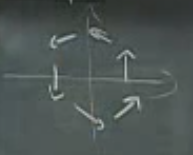
\includegraphics[height=3cm]{21_1.png}

Bir onceki derste bu alanin muhafazakar olmadigina (yani gradyan alani
olamayacagina) karar vermistik, cunku ustteki cember etrafinda bir cizgi
entegrali alinca sonuc sifir degil, pozitif bir deger cikiyordu. Ama biz
yine de, biraz once ogrendigimiz teknigi kullanarak bunu kontrol edelim.

\[ \vec{F} = \underbrace{-y}_{M}\hat{i} + 
\underbrace{x}_{N}\hat{j} 
\]

\[ \frac{\partial M}{\partial y} = -1 \]

\[ \frac{\partial N}{\partial x} = 1 \]

Bu iki sonuc birbirinin aynisi degil. Demek ki alan bir gradyan alani
degil. 

Ornek

\[ \vec{F} = (4x^2 + axy)\hat{i} + (3y^2 + 4x^2)\hat{j} \]

Hangi $a$ degerleri icin bu alan bir gradyan alani olur? 

\[ M_y = ax \]

\[ N_x = 8x \]

$a=8$. Bu arada, ikinci kismi turevleri birbirine esit yapinca, bu esitlik
her noktada dogru olmalidir. Yani cebirsel olarak bir esitlik hazirlayip
cebirsel numaralarla $x$'i bulmuyoruz, cunku cebirsel olarak cozumde $x=0$
da islerdi, ama bu dogru cevap olmazdi. Biz esitligin iki tarafinin
``tamamen ayni ifade'' olmasini istiyoruz.














\end{document}
